


\subsection{Introduction}
With its strong perception capabilities for navigation and obstacle avoidance in a variety of environments, mmWave radar technology has emerged as a key component in the development of mobile robotics. Radars operate in the 30 GHz to 300 GHz frequency range \citep{Skolnik2001}. The current state of the art is described in this section, with particular attention paid to its benefits, integration into robotic systems, operational principles, and state-of-the-art advancements in signal processing. For a comprehensive overview of radar principles and robotics applications, see \citep{Skolnik2001, Thrun2005}.

\subsection{Sources Analysis}
Bibliometric data analysis is an important stage for understanding the current state and development dynamics of the research area. This section presents an analysis of scientific publications indexed in the Scopus database on the topic of the application of millimeter waves (mmWave) and FMCW radars in robotics and autonomous systems.

The general methodology for conducting the source analysis followed a structured approach, as illustrated in Figure~\ref{fig:methodology_flowchart}. The process began with the \textbf{Start} or initiation of the research. This was followed by \textbf{Identify Keywords}, which involved determining relevant keywords and search terms crucial for a comprehensive literature search. This step included selecting terms related to millimeter-wave technology ("mmwave", "FMCW radar", "60 GHz") and its applications in robotics and autonomous systems ("robot", "UAV", "autonomous vehicle"). Subsequently, the step \textbf{Use the Keywords in Database Queries} involved applying the identified keywords to construct a search query for a comprehensive bibliographic database (Scopus in this case), which also included defining publication year constraints (2000-2025) to focus the search. The \textbf{Results from Queries} step led to the retrieval of an initial set of documents based on the executed query. A critical evaluation phase, \textbf{Results are according to the requirement?}, then assessed the relevance of the retrieved results to the research topic. This was an iterative step; if the results were not satisfactory (No), the process could revert to refining keywords or query parameters. If the results met the requirements (Yes), the \textbf{Selected Relevant Research Studies} were chosen for further analysis. Finally, the \textbf{End} marked the completion of the source selection phase, leading to the subsequent analysis of the selected documents, as detailed in the following sections.

\begin{figure}[H]
\centering

\includegraphics[width=0.5\textwidth]{Src/images/width_559.png}
\caption{General methodology for source analysis.}
\label{fig:methodology_flowchart}
\end{figure}

The search was performed using the following query: \texttt{TITLE-ABS-KEY ( ( "mmwave" OR "mm-wave" OR "millimeter wave" OR "FMCW radar" OR "60 GHz" ) AND ( "robot" OR "robotics" OR "mobile robot" OR "autonomous vehicle" OR "UAV" OR "drone" OR "AGV" ) ) AND PUBYEAR > 1999 AND PUBYEAR < 2026}. As a result, 2920 documents published between 2000 and 2025 were found. Key characteristics of this array of publications will be discussed below.

\subsubsection*{Dynamics of Publication Activity by Year}
The dynamics of publication activity by year (Figure~\ref{fig:years_png}) show a significant growth of interest in the topic. After a period of relatively low activity from 2000 to 2010 (averaging about 10 articles per year), the number of publications began to increase rapidly, especially after 2016. The peak of publication activity occurred in 2023 (503 publications) \citep{Kim2020MulRan}. In 2024, 415 articles were recorded, and preliminary data for 2025 (as of June) amount to 134 publications. The overall trend clearly demonstrates an exponential growth of research attention in this area over the last decade.

\begin{figure}[H]
\centering
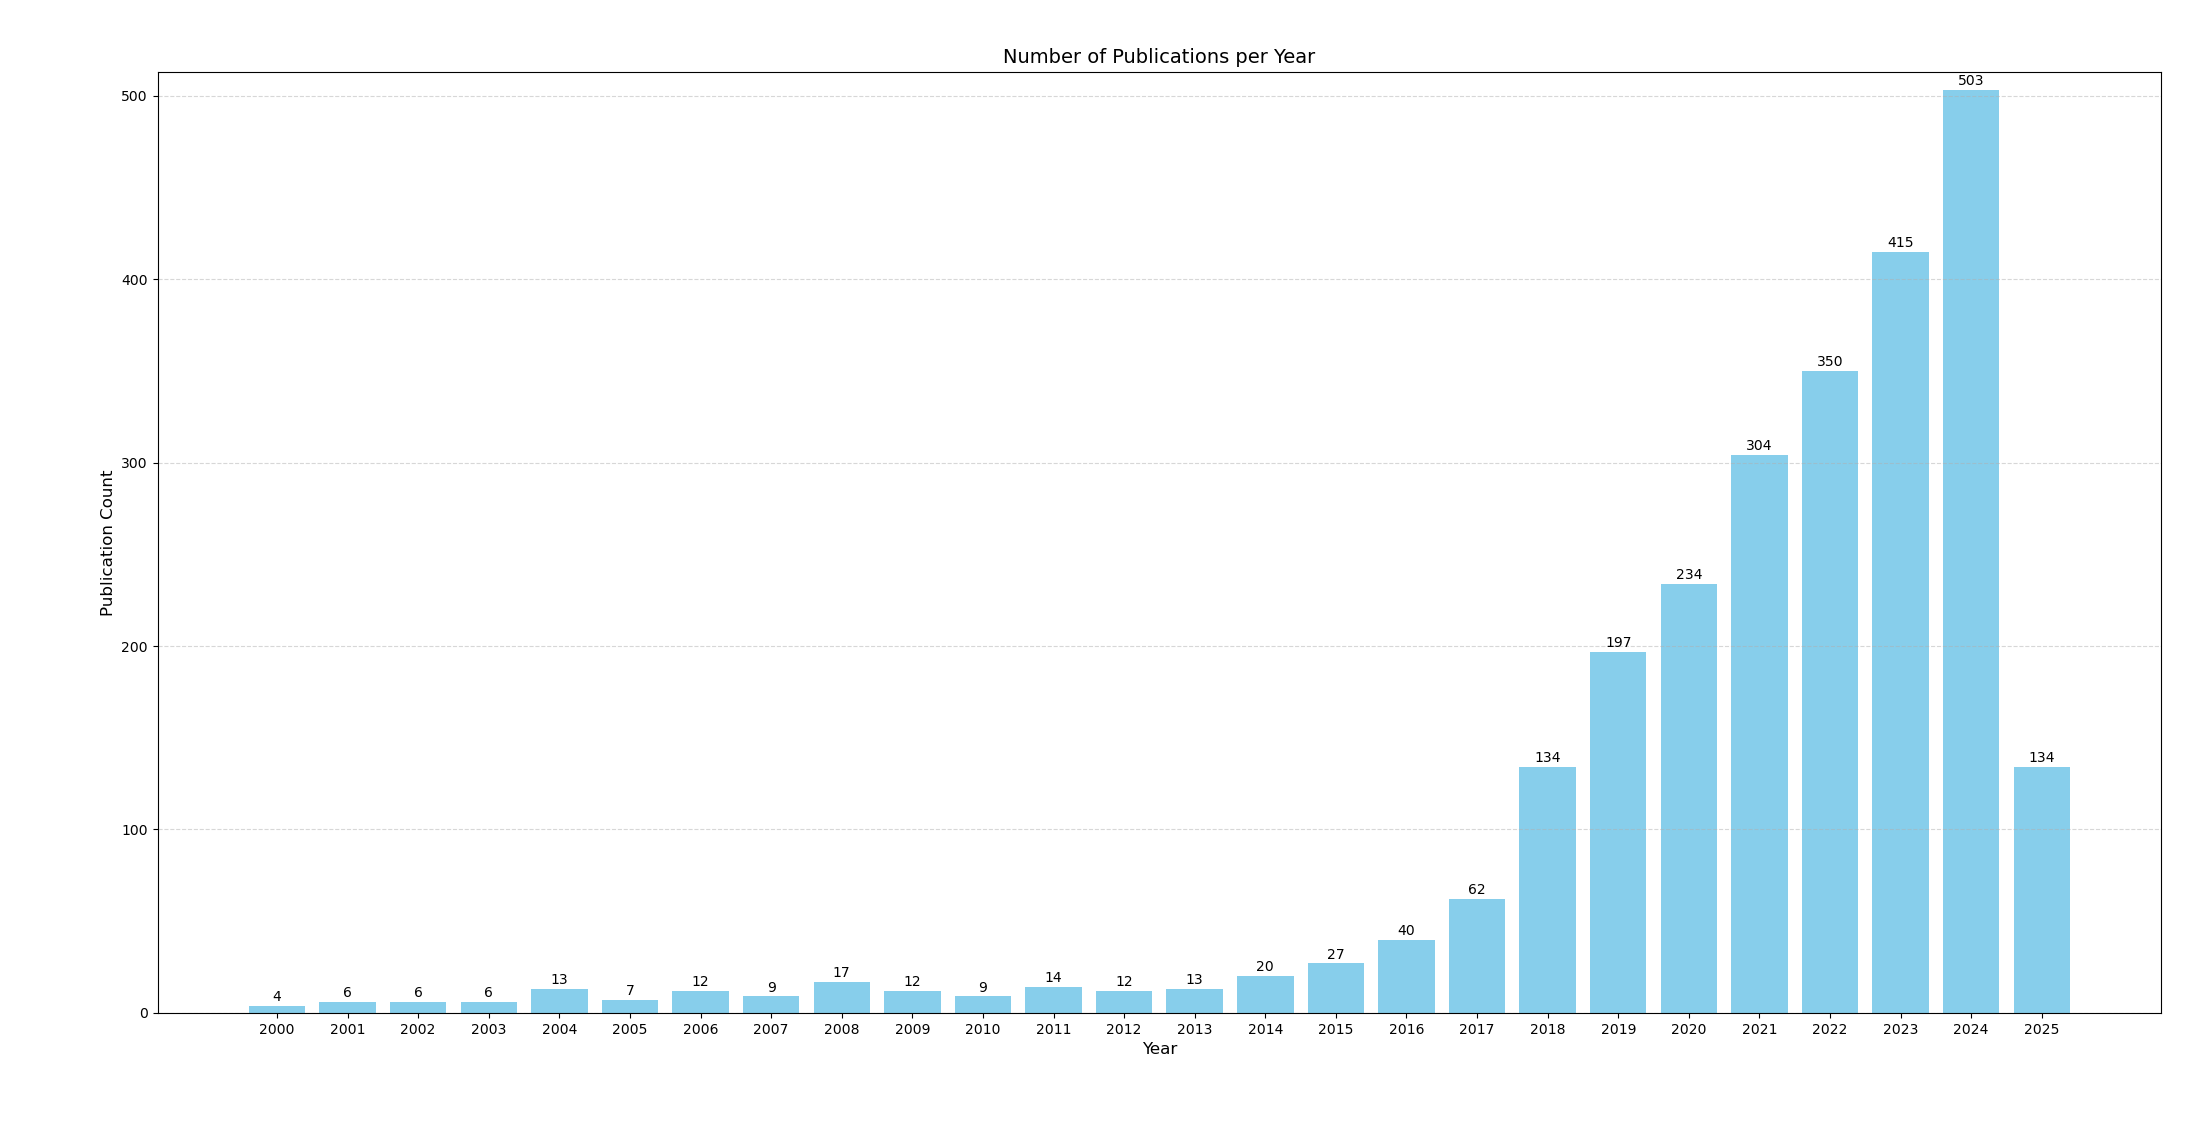
\includegraphics[width=\textwidth]{Src/images/Years.png}
\caption{Dynamics of publication activity by year.}
\label{fig:years_png}
\end{figure}

\subsubsection*{Distribution of Articles by Volume}
The distribution of articles by volume (Figure~\ref{fig:article_png}) revealed that publications of small volume are most common. The maximum number of articles (218) corresponds to 5-page works. Overall, there is a high concentration of articles ranging from 2 to 15 pages, while the number of more voluminous works (over 20 pages) is significantly smaller. This observation may indicate a high proportion of short communications or conference proceedings in the overall publication flow.

\begin{figure}[H]
\centering
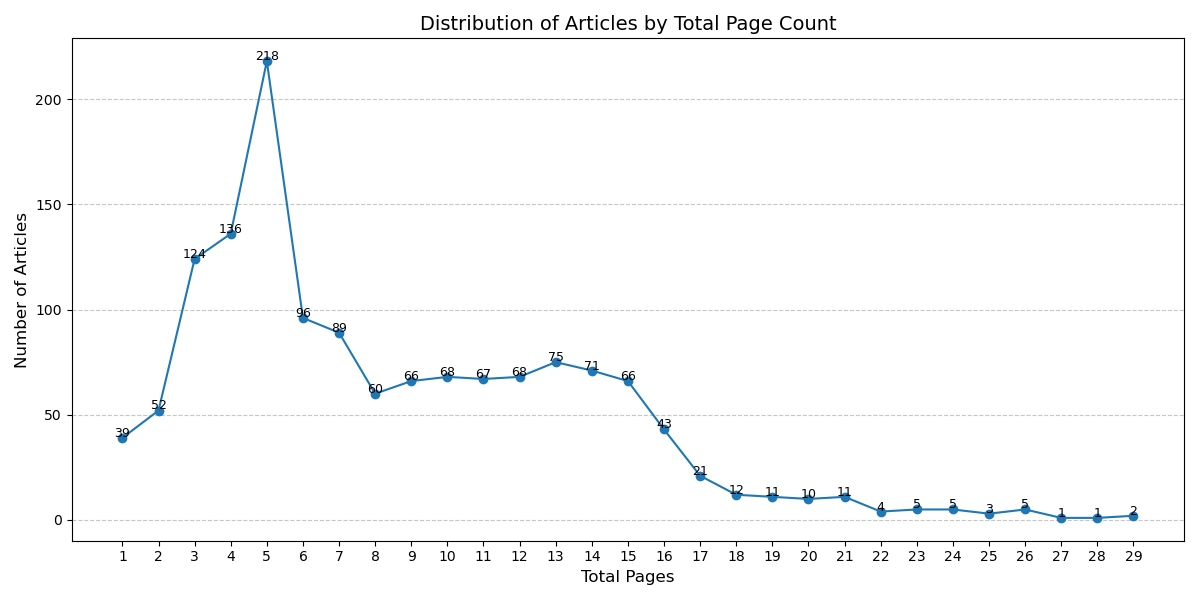
\includegraphics[width=1\textwidth]{Src/images/Article.png}
\caption{Distribution of articles by volume.}
\label{fig:article_png}
\end{figure}

\subsubsection*{Analysis of Publication Types}
The analysis of the types of publications (Figure~\ref{fig:output6_png}) further  the structure of the document array and confirms the previous conclusions. The dominant types are:
\begin{itemize}
    \item \textbf{Conference paper}: 48.9\%
    \item \textbf{Article}: 39.5\%
\end{itemize}
Together, these two types account for almost 88.4\% of all publications. A significantly smaller share is occupied by:
\begin{itemize}
    \item \textbf{Conference review}: 7.8\%
    \item \textbf{Review}: 2.3\%
    \item \textbf{Book chapter}: 1.0\%
    \item \textbf{Other}: 0.5\%
\end{itemize}
The predominance of conference papers and journal articles aligns with the rapid dissemination of research results in this field \citep{Thrun2005}.

\begin{figure}[H]
\centering
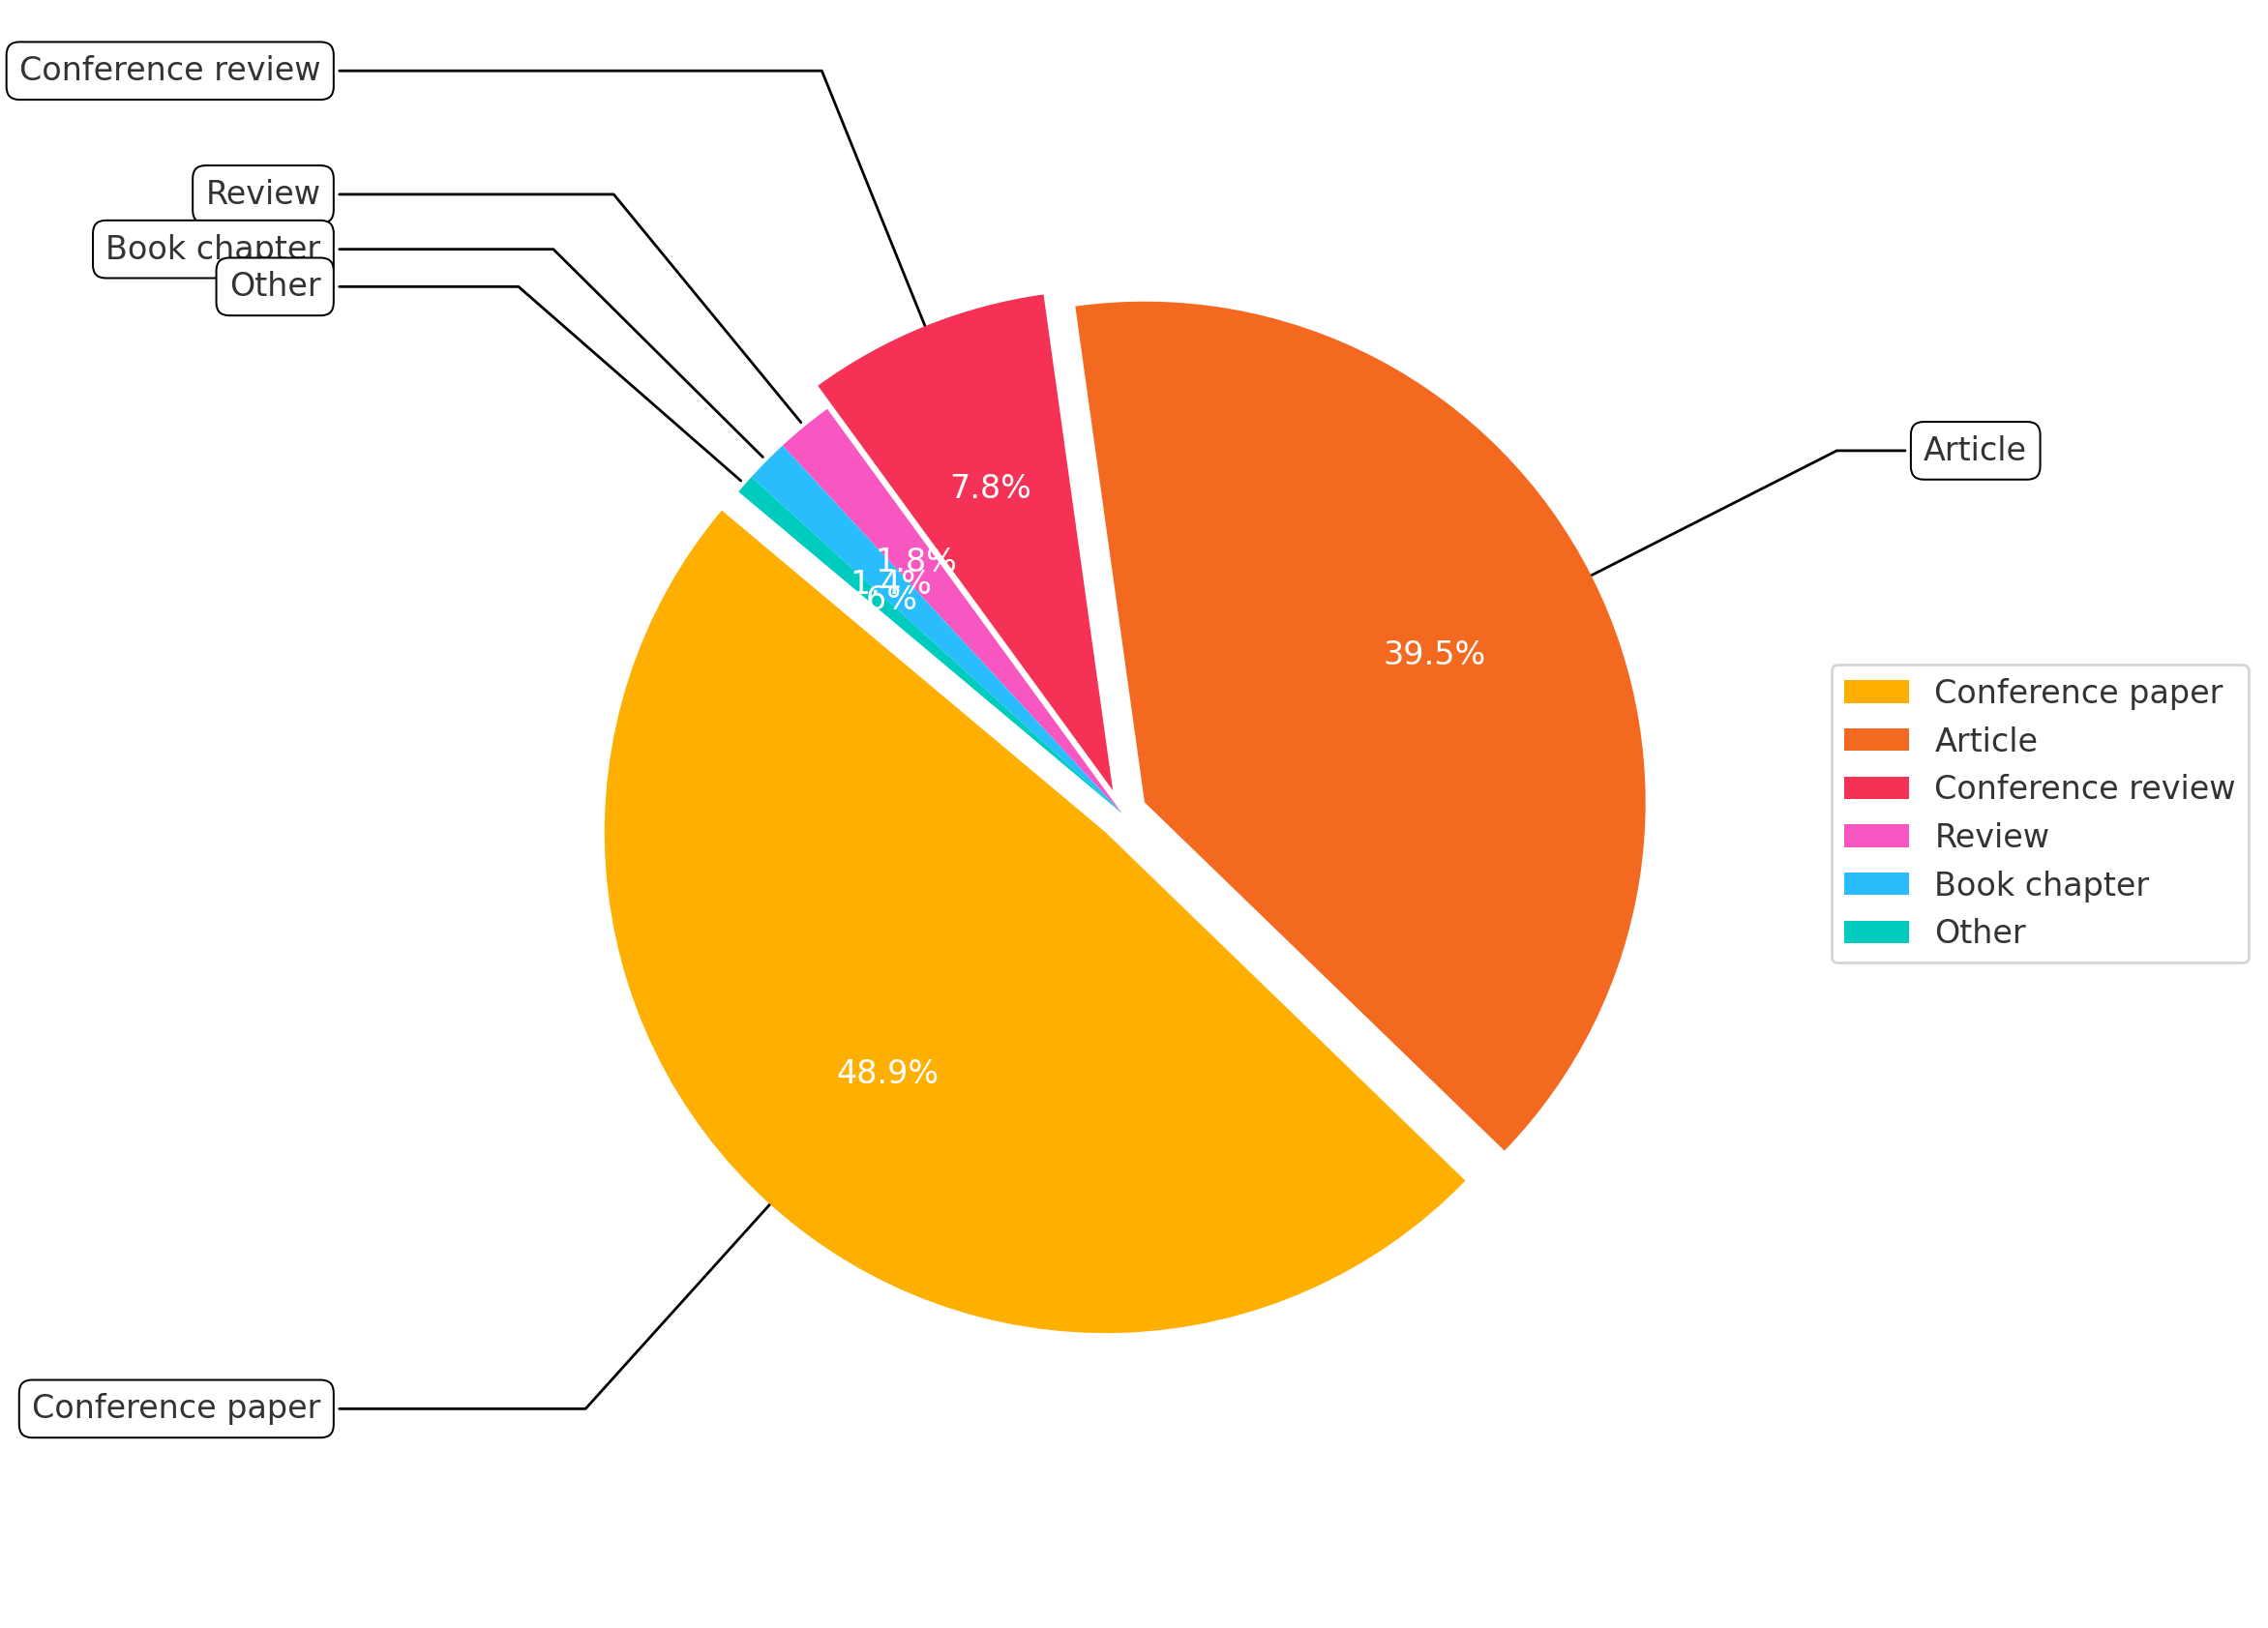
\includegraphics[width=0.65\textwidth]{output(6).png}
\caption{Analysis of publication types.}
\label{fig:output6_png}
\end{figure}

\subsection{Applications}


\noindent
In recent years, there has been a significant increase in the number of devices utilizing mmWave radars. 

\paragraph{Autonomous vehicles:}
In the automotive industry, millimeter wave radars have been incorporated for decades – they act as 'distant eyes' of the vehicle for advanced driver assistance systems (ADAS). A classic example - cruise control with radar: the front-mounted radar continuously measures the distance and speed of vehicles ahead, allowing the system to automatically adjust speed and maintain a safe distance. Radars are also employed for emergency braking in the event of obstacles, monitoring “blind spots”. For instance, Tesla (until 2021), combined a front-facing ~77 GHz radar with cameras, while many other manufacturers have added multiple radars around the vehicle for a comprehensive view. 
\paragraph{For research purposes:} 

The \textbf{Oxford RobotCar} project at Oxford University has garnered significant attention – a 2D laser (lidar) and a specialized 76 GHz frequency-modulated continuous wave (FMCW) radar (\textbf{Navtech CTS350-X scanning system}) have been installed on an unmanned standard vehicle.\citep{Barnes2020RadarRobotCar}
This radar system rotated 360 degrees, similar to a lidar system, and provided a radar image of the surroundings with a resolution of approximately \textbf{0.9 degrees} at a distance of \textbf{163 meters}   .
As a result, also a large dataset was collected for the \textbf{Oxford Radar Robot Car}. All sensors (camera, lidar, radar, and odometry) were recorded simultaneously as the vehicle traveled around the city.
This experiment confirmed that radar is suitable for large-scale urban mapping and navigation and remains operational even in challenging conditions such as rain, nighttime, and difficult lighting. Subsequently, several studies have been conducted using this data to develop algorithms for localization and obstacle avoidance based on radar images.
\paragraph{Other platforms:} 


Millimetre-wave radars are of interest for various applications, including unmanned aerial vehicles (UAVs), robotic manipulators and humanoid systems. For example, in the case of flying UAVs, radars can provide altitude measurements and detect obstacles such as smoke or dust, which is relevant for firefighting and military reconnaissance tasks. As part of the DARPA Subterranean Challenge, some teams experimented with radar technology for navigation in smoke-filled tunnels, where lidar sensors may be ineffective.

In humanoid robots, radars can help detect the presence and movement of people or objects that may be outside the camera's field of view. Texas Instruments has demonstrated a prototype in which a radar system located in the chest of the robot itself detects the presence and movements of a human, allowing the robot to respond appropriately even in low-light conditions, such as when a person has fallen and a response to that action is required.\citep{TI_SWRA831_2024}

\paragraph{In industrial robotics:} automated guided vehicles (AGVs) in factories and warehouse robots, radars are implemented to enhance safety. For instance, 60-64 GHz radar systems monitor the area surrounding a forklift truck, detecting people or other machinery and stopping the robot if a path is blocked.\citep{TI_RadarToolbox_Latest}
This technology can be applied across a wide range of platforms, from small household robots to vehicles, depending on their unique sensing capabilities.


\subsection{Public datasets and competitions}
Since the early 2020s, mmWave radars have increasingly been seen as an important component of autonomous vehicle and drone sensor systems. Their advantages, such as working in conditions of rain, fog, snow, dust, or total darkness, make them indispensable in scenarios where traditional optical sensors such as cameras and lidars are losing effectiveness. In addition, the development of compact and affordable radar chips, such as Texas Instruments solutions in various ranges, has contributed to their widespread adoption. However, to realize the potential of radars, not only hardware improvements are needed, but also high-quality data for training and testing algorithms. In response to this need, several significant open datasets have emerged in recent years that cover various scenarios, sensors, and operating conditions.

\begin{longtable}{|l|p{2cm}|p{3.5cm}|p{2cm}|>{\raggedright\arraybackslash}p{6.5cm}|}
    \caption{A summary of various radar-based datasets over the years.} \label{tab:radar_datasets} \\
    \hline
    \textbf{Year} & \textbf{Dataset} & \textbf{Sensor} & \textbf{Km/seasons} & \textbf{Features} \\
    \hline
    \endfirsthead

    \multicolumn{5}{c}%
    {{\bfseries \tablename\ \thetable{} -- continued from previous page}} \\
    \hline
    \textbf{Year} & \textbf{Dataset} & \textbf{Sensor} & \textbf{Km/seasons} & \textbf{Features} \\
    \hline
    \endhead

    \hline \multicolumn{5}{r}{{Continued on next page}} \\
    \endfoot

    \hline
    \endlastfoot

    2020 & Oxford Radar RobotCar & Navtech CTS350-X (360\textdegree) & 1000 km & Urban, rain/night \citep{10.1109/TRO.2024.3463504} \\ \hline
    2021 & MulRan               & Navtech HSC                       & 60 km    & Metropolis, fast driving \citep{9197298} \\ \hline
    2023 & Boreas               & CIR304-H (360\textdegree)         & 350 km, 4 seasons & Snow, fog, rain \citep{10.1177/02783649231160195} \\ \hline
    2024 & RadarScenes          & 77 GHz Continental                & 5 h      & Annotated occupancy grids \citep{10610514} \\ \hline

\end{longtable}


\subsection{Radar on chip}
Most existing solutions are represented by radar-on-chip systems. A radar-on-chip is an integrated system that combines radar functionality into a single compact microchip device (Figure \ref{fig:radarsensor}), making it applicable in various fields. Recent developments focus on replacing presence sensors (PIR), with the primary objective of detecting humans.\citep{s24113660}.

\begin{figure}[H]
    \centering
    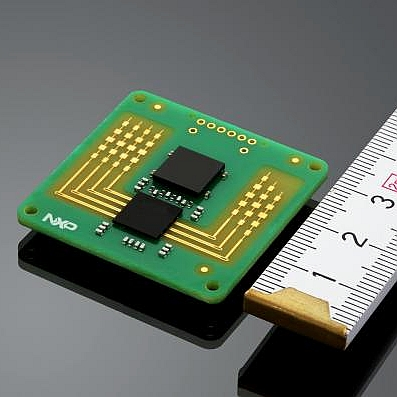
\includegraphics[width=\linewidth/2]{Src/images/automotive-radars.jpg} 
    \caption{Radar sensors \citep{ti_mmwave_overview}}
    \label{fig:radarsensor}
\end{figure}


\subsection{Signal processing}
The limitations of low-power radars in resolution (especially angular) and the abundance of noise have driven the development of specialized signal processing methods and perception algorithms. Since 2020, modern research has proposed various approaches to enhance the information content of radar data without significantly increasing equipment complexity \citep{Richards2010}. Key methods include filtering out noise and false alarms to improve detection reliability.

Indoors, radars generate numerous parasitic reflections, such as multipath "ghosts" and cloudy backgrounds \citep{Skolnik2001}. An essential step is applying a \textbf{CFAR filter} (constant false alarm rate) and other threshold algorithms directly on the radar chip to select significant reflections while suppressing noise \citep{Richards2010, Rohling1983}. The CFAR filter dynamically adjusts the detection threshold based on the local noise environment, ensuring robust target detection in challenging indoor settings \citep{Finn1986}.

\begin{figure}[h]
    \centering
    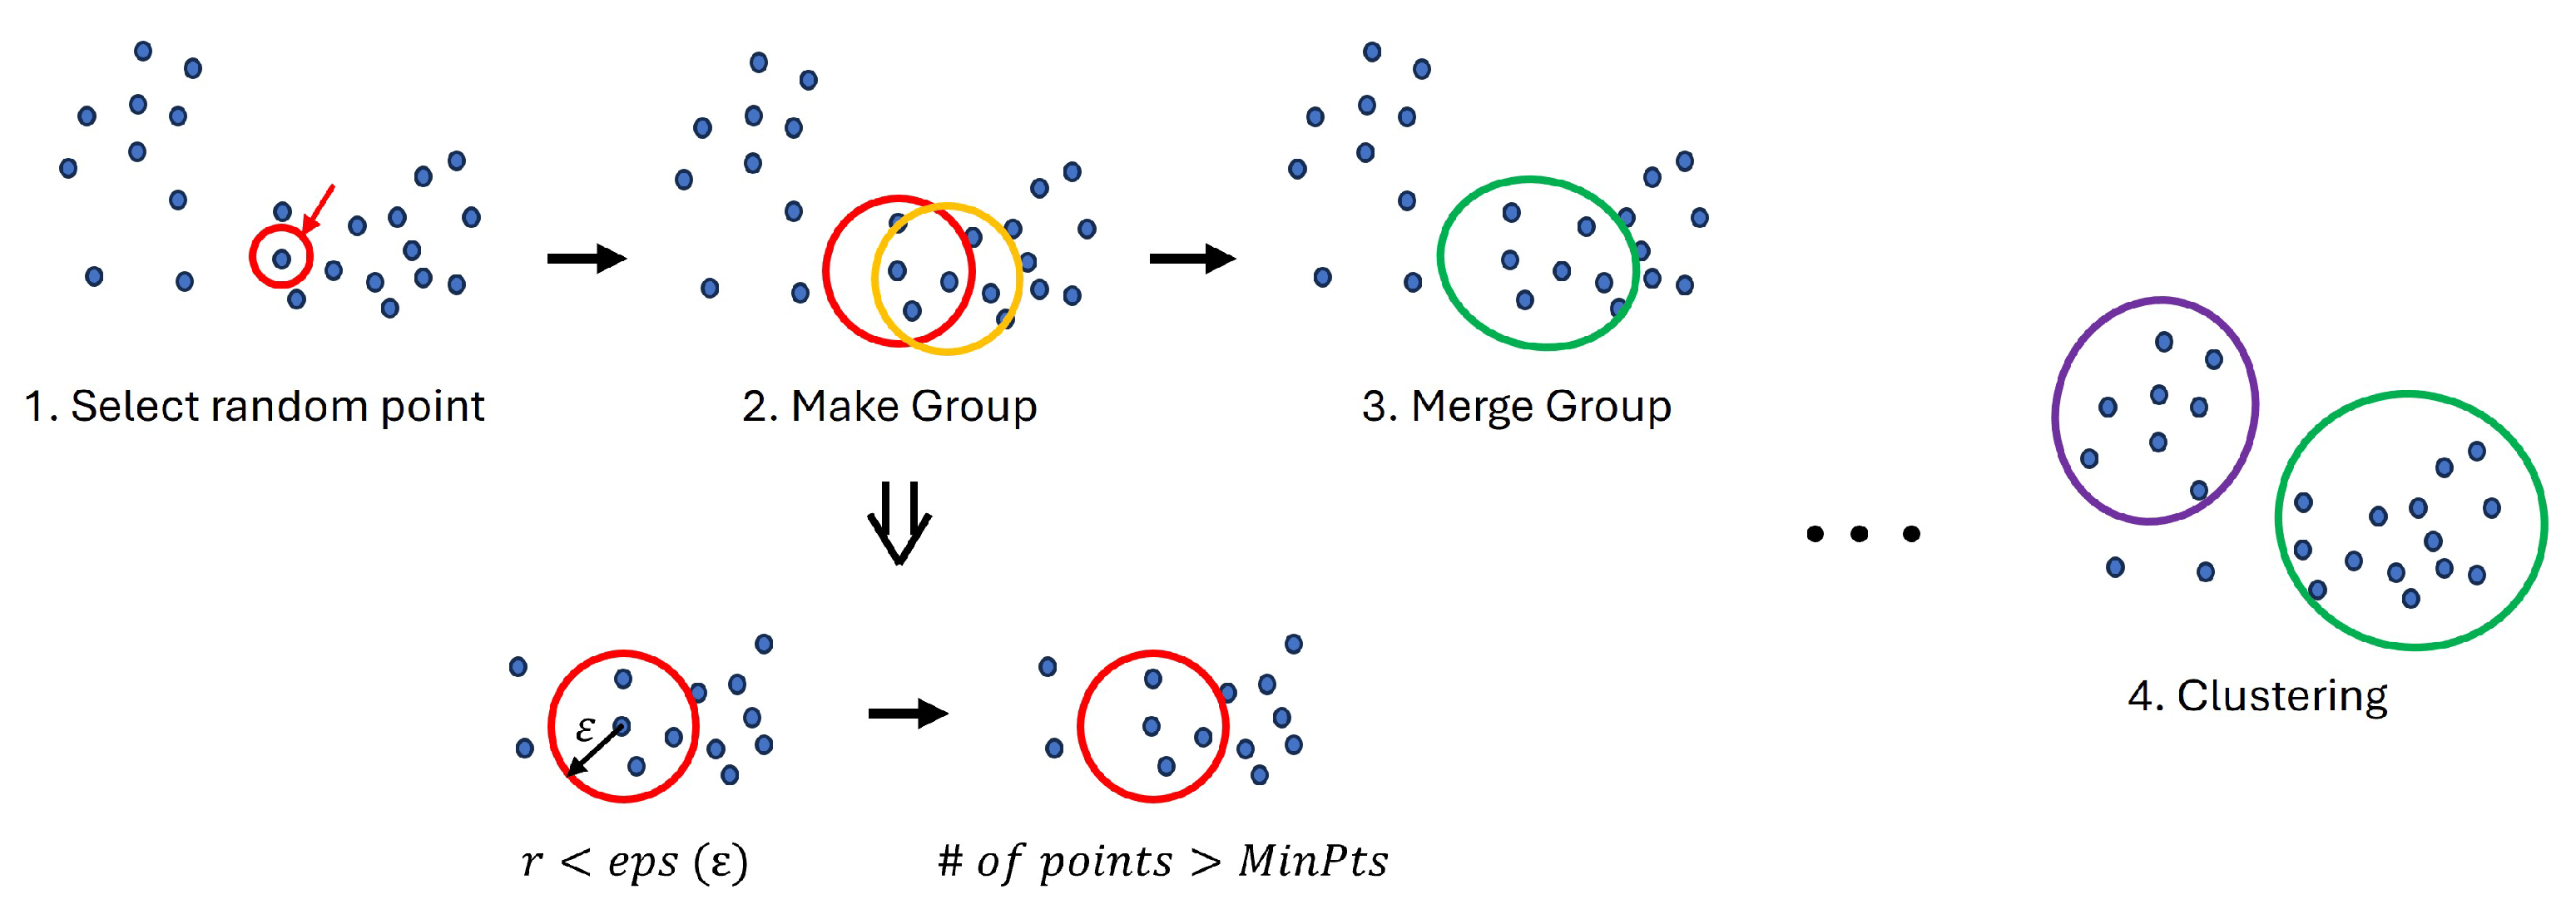
\includegraphics[width=\linewidth]{Src//images/electronics-13-03395-g001.png}
    \caption{DBSCAN illustration}
    \label{fig:DBSCAN}
\end{figure}

Further, \textbf{cluster filters} are applied at the application level: for example, methods like DBSCAN\ref{fig:DBSCAN}\citep{10.5555/3001460.3001507} are used to remove single outlier points and combine closely spaced reflections into one object. In addition, static can be filtered out by subtracting the background signal (as in Huang et al.). Another type of interference, speckle noise and periodic artifacts, is eliminated by averaging or identifying repeated patterns of false echoes.

\subsubsection{False point and noise filtering}
To enhance the resolution and address gaps in radar data, super-resolution algorithms, such as MUSIC (Multiple Signal Classification) or stable approximation methods, are commonly employed to improve the estimation of the angle of arrival (AoA) of the signal \citep{Schmidt1986, Richards2010}. These techniques mitigate the limitations of low angular resolution in low-power mmWave radars, enabling more precise target detection and localization.

The research community is actively exploring the capabilities of low-power mmWave radars for tasks such as mapping, obstacle detection, and avoidance of moving objects in robotic systems. One notable early project is the mmRanger system (2019), which utilized a pair of cost-effective 60 GHz communication modules installed on a consumer robot vacuum cleaner for environmental radar scanning \citep{Kumar2019mmRanger}. The robot exchanged millimeter-wave signals between the modules during movement and rotation, with algorithms identifying reflected paths to reconstruct a map of reflective objects (walls, obstacles). This approach enabled mmRanger to generate indoor maps without external infrastructure, enhancing navigation accuracy in line-of-sight and reflective conditions \citep{Kumar2019mmRanger}.

A further advancement is the milliMap project, which addresses the sparsity and noise in 60 GHz radar data using a generative learning approach \citep{Lu2020milliMap}. The authors employed an auxiliary lidar during neural network training to translate sparse radar observations into dense occupancy maps, achieving quality comparable to lidar. The resulting algorithm reconstructed a dense room map with an error of less than 0.2 m and annotated object semantics (walls, doors, elevators) with approximately 90\% accuracy, as illustrated in Figure~\ref{fig:milliMap} \citep{Lu2020milliMap}.

\begin{figure}
    \centering
    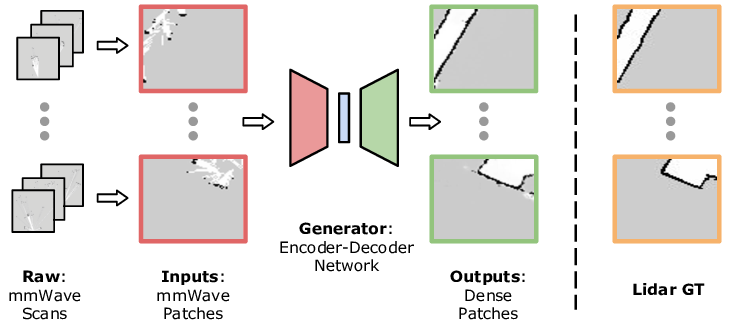
\includegraphics[width=0.75\linewidth]{Src/images/An-illustration-of-milliMap-A-neural-network-generator-takes-as-input-the-stitched.png}
    \caption{An illustration of milliMap \citep{lu2020smokerobustindoormapping}{}}
    \label{fig:milliMap}
\end{figure}

\subsubsection{Health monitoring}
Another area of research is contactless monitoring of vital signs (respiration and heartbeat) using mmWave. Since 2020, several prototypes have appeared, demonstrating that even a low-power radar can accurately measure a person's breathing rate and pulse from a distance. Thus, the mentioned Imec radar is specially optimized for high sensitivity for detecting small body movements \citep{imec_60ghz_radar_chip} In experiments, he showed the possibility of detecting heartbeats at 5 m and tracking the position and speed of human movement.


The research by \cite{elghitani2021automotive} is aimed at multi-targeted tracking of people indoors using radar: the algorithm successfully distinguishes up to 5 people and tracks their movement trajectories

Amazon is also interested in such radars – the company has requested regulatory approval to use 60-64 GHz radars on unmanned drones to survey the space around and prevent collisions in the air \citep{fcc_60ghz_policy}

%%%%%%%%%%%%%%%%%%%%%%%%%%%%%%%%%%%%%%%%%%%%%%%%%%%%%%%%%%%%%%%%%%%%%%%%%%%%%%%%%%%%%%
\subsection{Motion Planning}


Since the radar measures speed relative to itself, it is possible to estimate its own speed/odometry, similar to how wheels or visual sensors give odometry. RadarIzE\citep{10.1145/3643832.3661871} offers a full-fledged SLAM system using only one mmWave radar without IMU and wheel sensors. The authors point out that the radar has unique problems – the disappearance of objects due to specular reflections and “phantoms" due to multipath. As a result, the proposed SLAM approach significantly improved accuracy compared to previous ones: the odometry error was reduced by about 5 times, and the final SLAM trajectory error was reduced by 8 times (ATE metric) relative to other solutions.

One of the interesting studies in the role of path planning is \textbf{waveSLAM} \citep{picazo2023waveslam}, where two conventional 60 GHz communication modules \textbf{(WiGig)} are used instead of specialized radars While the robot is moving, the modules exchange signals, receiving reflections from surrounding surfaces, and build a map based on mutual measurements of range and angle. Although waveSLAM combines mmWave radio data with lidar, it is noteworthy that it has achieved an accuracy of ~22 cm in position and ~20° in orientation – comparable to lidar.


\subsection{Comparison of modern solutions}
\noindent
Radar-based solutions were analysed and presented in Table \ref{tab:radar_solutions}.

\begin{table}[h]
    \centering
    \small
    \caption{Overview of radar-based solutions and their applications}
    \label{tab:radar_solutions}
    \begin{tabular}{|p{1.5cm}|p{2.5cm}|p{2.5cm}|p{4cm}|p{4.5cm}|}
        \hline
        \textbf{Solution (Year)} & \textbf{Hardware Base} & \textbf{Task / Function} & \textbf{Approach} & \textbf{Results} \\ \hline

        milliMap  & 60 GHz single-chip radar + LiDAR (used only during training) & Indoor mapping, semantic object recognition in smoke & Generative model: joint processing of radar and LiDAR data during training & Dense map comparable to LiDAR (error < 0.2 m); $\sim$90\% classification accuracy through smoke. \\ \hline

        Huang et al., 2021 & TI IWR1642 (77 GHz, 2Tx/4Rx), low-power & Indoor human detection and tracking & Background removal, clustering, Kalman tracking on embedded system & Real-time tracking of 1–5 people (on Raspberry Pi); accuracy: 98\% (1 person) to 65\% (5 people), position error $\sim$0.3 m. \\ \hline

        Radarize& 60–77 GHz single-chip radar & Radar-only SLAM (no other sensors) & Doppler-based odometry + multipath suppression; map built from integrated radar points & Odometry error reduced by $\sim$5$\times$, SLAM (ATE) by $\sim$8$\times$ compared to previous approaches. \\ \hline

        waveSLAM  & 60 GHz WiFi AD radio + LiDAR & Indoor mapping (in glass/smoke environments) & FTM exchange between two mmWave radios; data merged with LiDAR & Accuracy: $\sim$\textbf{22 cm} position, 20\textdegree{} orientation; more robust than LiDAR in glass/fog conditions. \\ \hline

        Imec VitalRadar & 60 GHz AoP radar chip (7 GHz), 62 mW & Vital sign monitoring, movement tracking & Impulse FMCW (2 cm resolution), extraction of micro-movements & Detection of heartbeat at 5 m, hand gestures; ultra-compact (4.15 mm²), energy efficient. \\ \hline
    \end{tabular}

\end{table}


\subsection{Section conclusion}
MmWave radar has become a versatile sensor in numerous domains, including mobile robotics, autonomous vehicles, and healthcare, thanks to its resilience in challenging environments where cameras and lidars fail. Its capacity to measure velocity and self-motion has enabled its application in diverse fields, ranging from advanced driver assistance systems (ADAS) to warehouse robotics.
Public datasets, such as the Oxford Radar RobotCar, and competitions, such as the DARPA Subterranean Challenge, have contributed to advancements in simultaneous localization and mapping (SLAM), object recognition, and interference filtering. The integration of radar technology into chip-scale devices has reduced their size and power consumption, making them suitable for use in Internet of Things (IoT) and wearable devices. 
Algorithmic improvements, including CFAR filters, DBSCAN clustering, and super-resolution techniques, have enhanced mapping accuracy to approximately 0.2 meters and object classification through smoke to approximately 90\%.. 
However, challenges remain, such as multipath 'phantoms', calibration for sensor fusion, and the lack of standardized data formats. Future trends include hybrid radar and visual systems, broadband FMCW for subcentimeter resolution, and MIMO arrays supported by cloud and edge computing. Although millimeter-wave radars are a mature technology, addressing these shortcomings is important to expand their application domain.